\documentclass[english]{scrartcl}
\usepackage[T1]{fontenc}
\usepackage[utf8]{inputenc}
\usepackage[scaled=.8]{beramono}
\usepackage{geometry}
\geometry{verbose,tmargin=3cm,bmargin=3cm,lmargin=3cm,rmargin=3cm}
\usepackage{microtype}
\usepackage[parfill]{parskip}
\usepackage{amsmath}
\usepackage{graphicx}
\usepackage{hyperref}
\usepackage{nameref}
\usepackage{float}
\usepackage{listings}
\usepackage{color}
\usepackage{fancyhdr}
\usepackage{blindtext}

\usepackage{subcaption}
\usepackage{booktabs}

\pagestyle{fancy}
\fancyhf{}
\rhead{Group 2}
\lhead{DM: Subspace Clustering}
\cfoot{\thepage}

\newcommand*{\fullref}[1]{\hyperref[{#1}]{\autoref*{#1}~\nameref*{#1}}}

\definecolor{darkgray}{rgb}{0.66, 0.66, 0.66}
\definecolor{asparagus}{rgb}{0.53, 0.66, 0.42}

\lstdefinestyle{s}{
  commentstyle=\color{darkgray},
  keywordstyle=\bfseries,
  morekeywords={},
  stringstyle=\color{asparagus},
  basicstyle=\ttfamily\footnotesize,
  breakatwhitespace=false,
  keepspaces=true,
  numbersep=5pt,
  showspaces=false,
  showstringspaces=false,
}

\lstset{style=s}

\begin{document}

\title{Data Mining\\Programming Assignment 1: Subspace Clustering}

\author{Sonja Biedermann \and Thilo Hannes Fryen \and Chan Dat Dennis Huyen \and David Turner}

\maketitle
\tableofcontents

\section{ORCLUS}

We decided to implement the ORCLUS algorithm. ORCLUS is a spin on $k$-means
which utilizes eigensystems to adapt the distance measure to non axis parallel
correlation clusters.

We picked this algorithm because the paper is easy to read and contains good
pseudocode which is of utmost importance when trying to actually implement
the described algorithm.

Furthermore, since $k$-means was the first clustering algorithm we studied, it will forever
have a special Gaussian-shaped spot in our heart---which makes ORCLUS, as a
spiritual successor, a natural choice.

\subsection{Description and Pseudocode}

The algorithm proceeds in rounds in which the dimensionality of the clusters
and the number of clusters is gradually reduced. The rate at which this happens should
not be too quickly, to which end the authors propose two parameters $\alpha$ and $\beta$
and a relation between these two, by which one can be calculated from the other. They
suggest an $\alpha$ of 0.5, which we've also adopted.

In each round, the algorithm undertakes an assignment step which is the same as
in $k$-means. Every point is assigned to the closest centroid. However, as a
next step, the eigenvectors associated with the smallest spread are computed on
a per cluster basis---the rationale behind this is that those vectors define a
subspace in which the points cluster well, i.e. have a low contribution to the
overall cluster energy. The cardinality of this vector set dictates the dimensionality
of the subspace to which the points are projected.

To reduce the amounts of clusters---the algorithm starts with more seeds than
requested by the user, we've chosen to start with 5 times as many as the
authors offer no suggestions---a merging step is performed next. Although quite
lengthy, this operation is pretty simple. The objective is to find pairs of
clusters which can be merged such that the overall cluster energy stays low.
For this, all pairs of clusters are examined, their centroid and energy
computed and then the cluster-pairs with the lowest energy are picked to be merged, being
careful to update all relevant data structures after each merge.

These three steps are repeated until the desired dimensionality and number of
clusters are reached. After a final assignment step the clustering is returned.

%% TODO: pseudocode

\subsection{Implementation}

We chose to implement the algorithm in Python 3. The implementation is rather straight
forward and only depends on NumPy and some functionality from Python's standard
library.

Notably we use \texttt{numpy.linalg.eigh} to decompose the cluster matrices
into eigenvalues and eigenvectors. We know PCA could also be used but online
literature\footnote{\url{https://stackoverflow.com/questions/50358310/how-does-numpy-linalg-eigh-vs-numpy-linalg-svd}}
suggests that the LAPACK routines utilized in NumPy's implementation of
\texttt{eigh} perform a tiny sliver better than SVD, which we expect to be used
in \texttt{sklearn.decomposition.PCA}.  However, this probably would make no
practical difference whatsoever.

The initial seeds are distributed using the kmeans\texttt{++} initialization strategy,
although we have also implemented a completely random initalization strategy.
If the initial seed count is chosen to be high enough, this strategy actually
seems to be beneficial, as it returns good partitions and is also faster.

\section{Evaluation}

We will be comparing ourselves to the ELKI implementation on 4 synthetic datasets
using the NMI as scoring method. The datasets were generated using ELKI's data generator.
We used flat Gaussian distributions as correlation clusters and added noise points
to disturb the algorithm.

\subsection{Methodology}

The evaluation should be fully reproducible. File \texttt{eval.sh} contains the calls made to our
test scripts and ELKI. \texttt{summary.rb} is a Ruby script which processes the results, outputs
an overview table and also generates a \texttt{gnuplot}-ready plot file for plotting a boxplot of
the results.

We execute the test runs 5 times and note their resulting NMIs as well as the clusterings with the
best NMI score.

\subsection{Simple dataset}

As a simple first dataset we feed a 2-dimensional data set containing 3 clusters that are very clearly
separated, one of which is a bit fatter than the stereotypical correlation cluster, but which is
axis-parallel. Figure~\ref{fig:test} shows the results obtained by our implementation (Figure~\ref{fig:test-ours})
and the result obtained by the implementation contained in ELKI. They are identical---notably misclassifying one
single point which would belong to the fat axis-parallel cluster.

\begin{figure}[tb]
    \centering
    \begin{subfigure}[t]{0.5\textwidth}
        \centering
        \includegraphics[width=\textwidth]{img/test_ours}
        \caption{Our implementation}
        \label{fig:test-ours}
    \end{subfigure}%
    \begin{subfigure}[t]{0.5\textwidth}
        \centering
        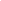
\includegraphics[width=\textwidth]{img/test_elki}
        \caption{ELKI's implementation}
    \end{subfigure}

    \caption{Bla}
    \label{fig:test}
\end{figure}

\subsection{Simple dataset with added noise}

We want to torment ORCLUS by adding noise to the previous trivial dataset.
It should perform much worse, since ORCLUS has no notion of noise by default
(and, although the authors recommend a simple scheme for implementing outlier
detection, this does not seem to be implemented in ELKI), but it is interesting
to see how the two implementation compare on a problematic dataset.

% coming soon

\subsection{Clusters that are noise in some subspaces}

It seems like a common situation in real-world data that clusters are present
in some subspaces, but are very dispersed in other subspaces, where other
clusters may reside---thus clusters in some subspaces are noise in others. We
would thus expect the algorithm to struggle.

% coming soon

\subsection{Clusters with different rotations in some subspaces}

The final dataset is somewhat based on the example of projected clusters
in the paper. This dataset has two rotated clusters in the first two dimensions,
and Gaussian noise in the last two dimensions. We expect the algorithm to
correctly focus on the leading two dimensions and discard the other two.

% coming soon

\subsection{Summary}

Table~\ref{tab:overview} shows the results of our evaluation. The minimum,
maximum and average over the 5 runs are shown split between our implementation
(DM) and the implementation available in ELKI.

Interestingly, our implementation appears to have a slight advantage over
ELKI's.  Notice especially the discrepancy with dataset \texttt{paper}, where
ELKI's implementation appears extremely unstable, while ours uncovers the
cluster structure perfectly without fail. The biggest difference in our
implementation is that we use a different initialization strategy, namely
kmeans\texttt{++}---this might result in our algorithm having an easier time
converging to a good minimum since the cluster centres are already
well-separated. However, our implementation performed better even when using a
random seed picking strategy---we suspect that perhaps the eigenvalue
decomposition is implemented differently, or we are just lucky. We also want to
note that we use fewer initial seeds than ELKI.

Figure~\ref{fig:box} shows a boxplot of the obtained NMI scores. A more stable implementation
would have a shorter box, i.e. less variance in the results.

\begin{table}[]\centering
  \begin{tabular}{lrrrcrrr}\toprule
     & \multicolumn{3}{c}{DM} & \phantom{abc} & \multicolumn{3}{c}{ELKI}\\
    dataset & min & max & avg & & min & max & avg\\ \midrule
    test & 0.987 & 0.987 & \textbf{0.987} & & 0.537 & 0.987 & 0.811\\
    test noisy & 0.536 & 0.66 & \emph{0.634} & & 0.537 & 0.659 & 0.634\\
    higher dimensional & 0.271 & 0.323 & \textbf{0.297} & & 0.188 & 0.356 & 0.258\\
    paper & 1.0 & 1.0 & \textbf{1.0} & & 0.005 & 1.0 & 0.559\\
  \bottomrule
  \end{tabular}
  \caption{Overview of results}
  \label{tab:overview}
\end{table}

\begin{figure}
    \centering
    \includegraphics[width=\textwidth]{img/boxplt}
    \caption{Boxplot illustrating stability}
    \label{fig:box}
\end{figure}

\end{document}
